
%%%%%%%%%%%%%%%%%%%%%%%%%%%%%%%%%%%%%%%%%%%%%%%%%%%%%%%%%%%%%%%%
% neměnit
%
\documentclass[a4paper,10pt,twocolumn]{article}
\usepackage{lmodern}
\usepackage[czech]{babel}
\usepackage[T1]{fontenc}
\usepackage[utf8]{inputenc}
\usepackage{graphicx}
\usepackage{float}
\usepackage[top=0.5cm,bottom=2cm,left=1cm,right=1cm]{geometry}
%
%%%%%%%%%%%%%%%%%%%%%%%%%%%%%%%%%%%%%%%%%%%%%%%%%%%%%%%%%%%%%%%%


%%%%%%%%%%%%%%%%%%%%%%%%%%%%%%%%%%%%%%%%%%%%%%%%%%%%%%%%%%%%%%%%
% dopište jméno článku,který aplikujete, svá jména, školní(!!!) emaily (emaiy jakol milasek328@seznam.cz apod. prosím ne...)
%
\title{Technická zpráva k semestrální práci z předmětu MI-ROZ \\ Vektor četností charakteristického otisku čočky}
\date{\today}
\author{Tomáš Chládek, chladto1 \\ chladto1@fit.cvut.cz}
%
%%%%%%%%%%%%%%%%%%%%%%%%%%%%%%%%%%%%%%%%%%%%%%%%%%%%%%%%%%%%%%%%


%%%%%%%%%%%%%%%%%%%%%%%%%%%%   TEXT   %%%%%%%%%%%%%%%%%%%%%%%%%%%%%%%%%%%%
%
%
\begin{document}
\maketitle
\begin{abstract}
Zpráva se zabývá identifikací osob na základě snímků duhovek. Vstupem jsou unifikované obrázky rozměru 600x100px. Pro klasifikaci je vybrán vektor četností charakteristického otisku čočky. Pro zadanou testovací množinu 814 fotografii se 75 lidmi dosahuje klasifikace 60\% přesnosti pro metodu kNN a poměr 50:50. Při poměru 70:30 ve prospěch testovacích dat dosahuje přesnosti 70\%.
\end{abstract}

%%%%%%%%%%%%%%%%%%%%%%%%%%%   UVOD   %%%%%%%%%%%%%%%%%%%%%%%%%%%%%%%%%%%%%
%
\section{Úvod}
Máme k dispozici dataset 814 fotografii čoček pro 75 lidí. Pomocí duhovky bychom měli být schopni unikátně identifikovat každou osobu na zemi. Vzhledem k rozdílným vlastnostem levého a pravého oka musíme vzít v potaz přes 15 miliard duhovek. Vlivem času může toto číslo výrazně růst neboť každý den se narodí 353,000 dětí.\cite{worldPopupation} Vektor vlastností, který budeme extrahovat musí být tedy dostatečně robustní, aby tuto skutečnost reflektoval.\par
Obrázek se skládá ze 3 barevných spekter červené, zelené a modré. Každé spektrum můžeme využít k získání určité informace. V našem případě se snažíme získat robustní klasifikátor, který bude fungovat i za neideálních podmínek. To znamená, že snímky nejsou ideálně osvícené a kvalita se razantně liší. Na snímcích jsou nemalé části kůže nebo řas, které musí být odstraněny. Dále vzhledem k různým podmínkám pořízení snímku musí klasifikátor eliminovat odlesky a reflexi okolí.\par
Proto jsem se rozhodl nejprve upravit data do takové míry, aby byly od těchto nechtěných faktorů odstíněny. Tuto část nazývám preprocessing. Poté dojde k samotné klasifikaci obrázků, tedy vytvoření charakteristického vektoru. Jakmile je vytvořen dataset s klasifikacemi dochází k učení modelu. \par
Jednotlivé části procesu byly optimalizovány pro lepší výsledky. Poznatky z optimalizace jsou shrnuty na konci této zprávy.


\section{Předzpracování}

Dataset je již předzpracovaný, avšak k výše zmíněným nedostatkům je zapotřebí provést následnou úpravu. Průměrný obrázek vypadá asi následovně.
\begin{figure}[H]
       \begin{center}
              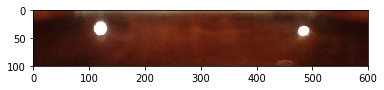
\includegraphics[width=6cm]{image_raw.png}
       \end{center}
       \caption{Jedná se o duhovku, která je na pevně definovaném místě rozkrojena do poloměru. Odsud je poté rozvinuta do obdélníku fixní délky.}
       \label{fig1}
\end{figure}

Zde si můžeme všimnout, že nejzřetelnější část je uprostřed. Dva bílé kruhy jsou důsledek reflexe světla při snímání obrázku. Pro úpravu tedy nejprve odřízneme krajních 150px na šířku z každé strany. Poté se podíváme na jednotlivá barevná spektra.

\begin{figure}[H]
      \begin{center}
            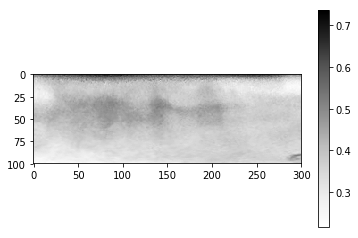
\includegraphics[width=6cm]{image_crop_red.png}
            \vspace{1mm}  
      \end{center}
      \caption{Zde je vidět výřez obrázku v červeném spektru. Ostatní spektra nesou jen málo informace o  textuře duhovky.}
\label{fig2}
\end{figure}

V červeném spektru vidíme určité rysy samotné duhovky. Tuto informaci se následně pokusíme co možná nejvíce separovat od zbytku. Zbylá spektra budeme pro teď ignorovat, neboť nenesou mnoho informací o otisku duhovky. Na horním okraji vidíme jasně tmavou linii. To je kus kůže, který musí být odstraněn před klasifikací. \par
V červeném spektru se nejprve pokusíme zvýraznit otisk duhovky. Spočteme si median a standardní deviaci. To nám vymezí rozsah hodnot, které pro nás mají smysl. Data mimo tento rozash budou brána jako nejblížší krajní hodnoty. Poté provedeme normalizaci, kdy spodní hranice je nula.

\begin{figure}[H]
      \begin{center}
            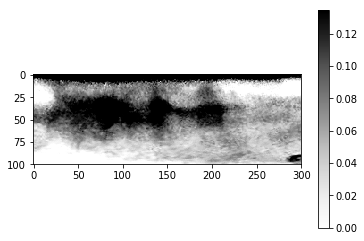
\includegraphics[width=6cm]{normalized_red.png}
            \vspace{1mm}  
      \end{center}
      \caption{Otisk duhovky je zvýrazněn}
\label{fig3}
\end{figure}
Když máme texturu jasně vymezenou můžeme provést selekci dat, které definují texturu. K tomu jsem zvolil selekci 30\% nejvýraznějších bodů, což jsou na originálním obrázku ty světlejší. Díky tomu dostaneme jasnou texturu duhovky.\par
K odstranění kůže z horní části obrázku použijeme modrého a zeleného spektra, které jsme do teď ignorovali. Vezmeme každé spektrum. Provedeme stejný proces jako s červeným spektrem pouze nás bude zajímat 10\% největších hodnot. Tyto hodnoty následně odečteme od červeného spektra a dostaneme očištěné červené spektrum. Výsledek pak jen začistím medianovým filtrem s parametrem 5, abychom se zbavili šumu, který vznikl.

\begin{figure}[H]
      \begin{center}
            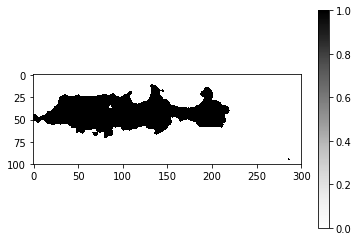
\includegraphics[width=6cm]{mask_diff.png}
            \vspace{1mm}  
      \end{center}
      \caption{Výsledek, který je určen ke klasifikaci.}
\label{fig5}
\end{figure}

%==================================    příznaky   ==================================================

\section{Klasifikace}

Pro klasifikaci byl vybrán vektor četností charakteristického otisku duhovky. Z každého sloupečku je brán počet tmavých bodů, které prošli preprocessingem. Jako učící model byl vybrán model KNN, neboť testovaný dataset je malý, a lze proto lehce udržet takovéto množství výsledků v paměti.

\section{Výsledky}
Délka výpočtu netrvá déle než 5 minut, což na jeden obrázek dělá zhruba 0.3s. Do tohoto času je započteno načtení a uložení obrázku na disk. Vyhodnocení obrázku je tedy velmi rychlé. Samozřejmě pro větší dataset by výpočet trval déle. Při výše definovaném postupu jsem dosáhl výsledků 70\% přesnosti při rozdělení 70:30. V zadání však bylo vyžádáno rozdělení datasetu na 50:50. Tímto se přesnost snížila na 60\%. Přesnost byla měřena při 100 náhodných rozdělení datasetu dle definovaného poměru. Dále jsem optimalizoval množství sousedů pro učící model. Zde chyba velmi rychle rostla a nejvhodnější parametr byl 1 pro všeschny testované množiny.\par
Vzhledem k předzpracování obrázku jsou již obrázky částečně centrovány. Horizontální normalizace vektoru zarovnáním doleva na první nenulovou hodnotu dosahovala horších výsledků. Zřejmě proto, že je důležité, kde se charakteristický otisk nalézá v prostoru. Drobné posunutí nevytvoří tak velkou chybu, jako kdybychom otisk zlevé strany přehodili na pravou stranu. Vertikální vertikace není zapotřebí, neboť v tomto směru nás zajímá pouze četnost. Využití modrého a zeleného spektra k odstranění řas, kůže a reflexe významně zvýšilo přesnost odhadu.\par
U obrázků není problém se změnou velikostí otisků, ani jejich rotací nebo změně barvy. Samozřejmě vlivem zpracování dojde k drobým transformacím, ale ty mohou být opraveny. Vliv osvícení oka výrazně mění barvu oka. Proto není doporučeno pracovat přímo s hodnotami pixelů.

\section{Možné rozšíření}

Navrhnutý postup je pouze ukázkou, že tento směr má solidní výsledky a jistě je možné ho ještě zlepšit. Například samotná selekce otisku duhovky je závislá na dvou parametrech, které nevyhovují všem výsledkům. Při optimalizaci této části lze ještě lépe vymezit samotný otisk a dosáhnout mnohem lepších výsledků. Stává se totiž že občas nám zůstane část kůže na obrázku nebo jsou body odebrány z otisku.\par
V případě zvětšení datasetu je možné vzít v potaz i vertikální četnost. V tuto chvíli však musíme dát pozor na rotaci a posun oka, neboť pozice není vždy stejná a tak může být zapotřebí dovylepšit posunutí. Navíc obrázek nemá stejně velké dimenze, takže by muselo dojít k určitému ohodnocení vlastností.\par 
Odstranění irelevantních částí z obrázku pomocí zbylých barevných spekter může být provedeno ještě před samotnou selekcí otisku, a tím může být selekce normalizována na fixní rozsah, kde mohou být následně data lépe vybrána. Může se jedna o určitou hodnotu, jakou otisk musí mít místo pouhého počtu položek.

%%%%%%%%%%%%%%%%%%%%%%%%%%   SHRNUTÍ   %%%%%%%%%%%%%%%%%%%%%%%%%%%%%%%%%%%
%
\section{Shrnutí}

Díky předzpracování obrázku bylo možné dosáhnout primitivní klasifikací velmi dobrých výsledků. Navrhnuté řešení není ideální pro globální řešení, neboť klasifikační model by bylo jen těžko možné udržet rychlý a škálovatelný. Dále vzhledem ke kvalitě obrázků a relativně očekávatelné distribuci vzorů by nám mohlo velmi rychle dojít ke konfliktům. To znamená, že náš vektor vlastností by musel být výrazně větší a složitější.
%
%%%%%%%%%%%%%%%%%%%%%%%%%%%%%%%%%%%%%%%%%%%%%%%%%%%%%%%%%%%%%%%%%%%


%%%%%%%%%%%%%%%%%%%%%%%%%%%   REFERENCE   %%%%%%%%%%%%%%%%%%%%%%%%%%%%%%%%%
%
\bibliographystyle{unsrt}
\bibliography{roz-TZ}

%%%%%%%%%%%%%%%%%%%%%%%%%%%%%%%%%%%%%%%%%%%%%%%%%%%%%%%%%%%%%%%%%%%
%
%
%%%%%%%%%%%%%%%%%%%%%%%%%%   END OF TEXT   %%%%%%%%%%%%%%%%%%%%%%%%%%%%%%%%%%

\end{document}
